\documentclass[11pt,a4paper]{article}
\usepackage[utf8]{inputenc}
\usepackage[T1]{fontenc}
\usepackage[a4paper]{geometry}

\usepackage{amsthm}
\newtheorem{theo}{Theorem}
\newtheorem{defi}[theo]{Definition}
\newtheorem{prop}[theo]{Proposition}

\usepackage{amssymb}
\usepackage{amsmath}
\usepackage{bbm}
\usepackage{stmaryrd}
\usepackage{proof}
\usepackage{tikz}
\usetikzlibrary{matrix}
\usetikzlibrary{decorations.pathmorphing}

\setlength\parindent{0pt}

\newcommand{\La}{\mathcal{L}}
\newcommand{\M}{\mathcal{M}}
\newcommand{\ph}{\varphi}
\newcommand{\itemz}{\item[$\triangleright$]}
\newcommand{\F}{\mathcal{F}}
\newcommand{\gr}{\textbf}
\newcommand{\il}{\textit}
\newcommand{\N}{\mathbb{N}}
\newcommand{\U}{\mathcal{U}}
\newcommand{\equi}{\Leftrightarrow}
\newcommand{\R}{\mathcal{R}}
\newcommand{\C}{\mathcal{C}}
\newcommand{\I}{\mathcal{I}}
\renewcommand{\iff}{\Leftrightarrow}
\newcommand{\T}{\mathbb{T}}
\newcommand{\V}{\mathcal{V}}
\newcommand{\lb}{\llbracket}
\newcommand{\rb}{\rrbracket}
\newcommand{\info}[1]{\text{{\fontfamily{lmss}\selectfont #1}}}
\newcommand{\List}{\info{List}}
\newcommand{\Tree}{\info{Tree}}
\newcommand{\1}{\mathbbm{1}}
\renewcommand{\contentsname}{Table des matières}
\renewcommand{\proofname}{Preuve}
\renewcommand{\P}{\mathcal{P}}
\newcommand{\Leaf}{\info{Leaf}}
\newcommand{\Node}{\info{Node}}


\usepackage[bitstream-charter]{mathdesign}
%\usepackage[charter]{mathdesign}
%\usepackage{fontspec}
%\setmainfont{URW Palladio L}
\title{Category theory and data structures}
\usepackage{multicol}

\begin{document}

\section{Category theory}
Is everything a map? No. Everything is a commutative diagram.
\begin{defi}[Category]
A category $\gr{C}$ is composed of a set of objects and sets of morphisms. For each objects $A,B$, there is a set of morphisms from $A$ to $B$. Morphisms are denoted by $f : A \to B$. There is a composition law $\circ$ and for each object $A$ there is an identity morphism $id_A : A \to A$ such that
\begin{itemize}
\setlength\itemsep{-0.3em}
\itemz $\circ$ is associative: $h \circ (g \circ f) = (h \circ g) \circ f$.
\itemz $id$ is neutral: $f \circ id_A = id_B \circ f = f$.
\end{itemize}
\end{defi}

\begin{center}
\begin{tikzpicture}
  \matrix (m) [matrix of math nodes,row sep=3em,column sep=4em,minimum width=2em]
  {
     A & B & C & D & & A & A \\
       &   &   &   & & B & B \\};
  \path[-stealth]
    (m-1-1) edge node [above] {$f$} (m-1-2)
    (m-1-2) edge [dashed] node [above] {$g$}(m-1-3)
    (m-1-3) edge node [above] {$h$} (m-1-4)
    (m-1-1) edge [bend left] node [above] {$g \circ f$} (m-1-3)
    (m-1-2) edge [bend right] node [below] {$h \circ g$} (m-1-4)
    (m-1-6) edge node [above] {$id_A$} (m-1-7)
    (m-1-7) edge node [right] {$f$} (m-2-7)
    (m-1-6) edge node [left] {$f$} (m-2-6)
    (m-2-6) edge node [below] {$id_B$} (m-2-7)
    (m-1-6) edge node [above right] {$f$} (m-2-7) ;
\end{tikzpicture}
\end{center}

\gr{Examples.}
\begin{itemize}
\setlength\itemsep{-0.3em}
\itemz $\gr{Set}$, objects are sets, morphisms are functions.
\itemz $\gr{Grp}$, objects are groups, morphisms are group homomorphisms.
\itemz $\gr{Vect}_K$ ($K$ is a field), objects are $K$-vector spaces, morphisms are $K$-linear applications.
\end{itemize}

\begin{defi}[Functor] Let $\gr{C}$ and $\gr{D}$ be categories. A functor $F : \gr{C} \to \gr{D}$ is a map that associates to each object $A \in \gr{C}$ an object $F(A) \in \gr{D}$, and to each morphism $f : A \to B$ in $\gr{C}$ a morphism $F(f) : F(A) \to F(B)$ in $\gr{D}$. A functor satisfies $F(g \circ f) = F(g) \circ F(f)$.
\end{defi}
\begin{center}
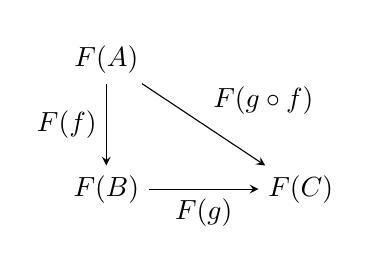
\begin{tikzpicture}
  \matrix (m) [matrix of math nodes,row sep=3em,column sep=4em,minimum width=2em]
  {
     F(A) &  \\
     F(B) & F(C) \\};
  \path[-stealth]
    (m-1-1) edge node [left] {$F(f)$} (m-2-1)
    (m-2-1) edge node [below] {$F(g)$}(m-2-2)
    (m-1-1) edge node [above right] {$F(g\circ f)$} (m-2-2);
\end{tikzpicture}
\end{center}

\gr{Examples (in \gr{Set}).} \begin{itemize}
\itemz The "$1+-$" functor is defined by $F(A) = 1 + A$ (the disjoint union of $A$ and a set with exactly one element $1 = \{*\}$), and if $f : A \to B$, then $F(f) = id_1 + f$ (i.e. $F(f)(*)=*$ and $F(f)(a) = f(a)$ for $a \in A$).
\itemz Let $C$ be a set. The "$C\times -$" functor is defined by $F(A) = C \times A$ (the cartesian product), and if $f : A \to B$, then $F(f) = id_C \times f$ (i.e. $F(f)(c,a) = (c,f(a))$ for $c \in C$, $x \in X$).
\end{itemize}
The composition of two functors is a functor.
\begin{defi}[Initial object]
Let $\gr{C}$ be a category and $A$ an object. $I$ is an initial object if for any object $A$ there exists exactly one morphism $\lb A \rb : I \to A$.
\end{defi}
\newpage
\section{$F$-algebras}
Now we know what is a category and what is a functor. These are the only tools we need in order to formalize properly mathematical induction, through what is called $F$-algebras.
\begin{defi}
Let $\gr{C}$ be a category and and $F : \gr{C} \to \gr{C}$ be a functor. (Note that this is an endofunctor: the domain category is the same as the codomain category.) An $F$-algebra is a morphism $\alpha : F(A) \to A$, where $A$ is an object of $\gr{C}$ called the carrier of $\alpha$.
\end{defi}
\begin{defi} Let $\alpha : F(A) \to A$ and $\beta : F(B) \to B$ be two $F$-algebras. A homomorphism of $F$-algebras from $\alpha$ to $\beta$ is a morphism $h : A \to B$ such that $\beta \circ F(h) = h \circ \alpha$.
\end{defi}
\begin{center}
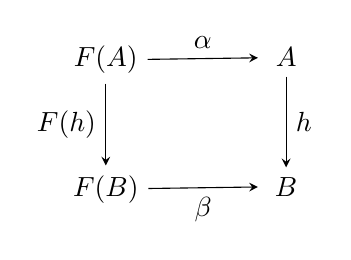
\begin{tikzpicture}
  \matrix (m) [matrix of math nodes,row sep=3em,column sep=4em,minimum width=2em]
  {
     F(A) & A \\
     F(B) & B \\};
  \path[-stealth]
    (m-1-1) edge node [left] {$F(h)$} (m-2-1)
    (m-2-1) edge node [below] {$\beta$}(m-2-2)
    (m-1-1) edge node [above] {$\alpha$} (m-1-2)
    (m-1-2) edge node [right] {$h$} (m-2-2);
\end{tikzpicture}
\end{center}
\begin{prop}
The $F$-algebras and their homomorphisms form a category denoted by $\gr{Alg}(F)$.
\end{prop}
\begin{proof}[Proof] Homework. Let us just prove that composing two $F$-algebra homomorphisms defines an $F$-algebra homomorphism. Proof by diagram:
\begin{center}
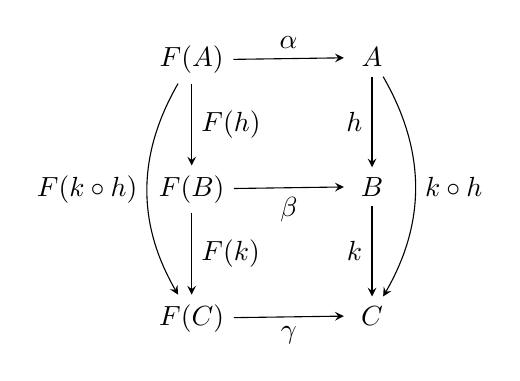
\begin{tikzpicture}
  \matrix (m) [matrix of math nodes,row sep=3em,column sep=4em,minimum width=2em]
  {
     F(A) & A \\
     F(B) & B \\
     F(C) & C \\};
  \path[-stealth]
    (m-1-1) edge node [right] {$F(h)$} (m-2-1)
    (m-2-1) edge node [below] {$\beta$}(m-2-2)
    (m-1-1) edge node [above] {$\alpha$} (m-1-2)
    (m-1-2) edge node [left] {$h$} (m-2-2)
    (m-2-1) edge node [right] {$F(k)$} (m-3-1)
    (m-3-1) edge node [below] {$\gamma$} (m-3-2)
    (m-2-2) edge node [left] {$k$} (m-3-2)
    (m-1-1) edge [bend right] node [left] {$F(k \circ h)$} (m-3-1)
    (m-1-2) edge [bend left] node [right] {$k\circ h$} (m-3-2);
\end{tikzpicture}
\end{center}
\end{proof}
If there exists an initial object in $\gr{Alg}(F)$, then it is of great importance. Unfold the definitions to see what it means to be an initial object in $\gr{Alg}$.\\\\
$\iota : F(I) \to I$ is initial if for any other $\alpha : F(A) \to A$ there exists a unique morphism $\lb \alpha \rb : I \to A$ such that the following diagram commutes.
\begin{center}
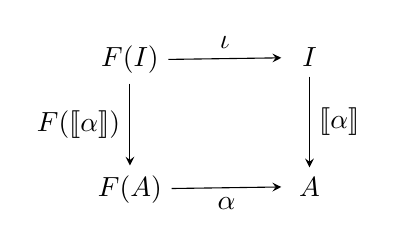
\begin{tikzpicture}
  \matrix (m) [matrix of math nodes,row sep=3em,column sep=4em,minimum width=2em]
  {
     F(I) & I \\
     F(A) & A \\};
  \path[-stealth]
    (m-1-1) edge node [left] {$F(\lb \alpha \rb)$} (m-2-1)
    (m-2-1) edge node [below] {$\alpha$}(m-2-2)
    (m-1-1) edge node [above] {$\iota$} (m-1-2)
    (m-1-2) edge node [right] {$\lb \alpha \rb$} (m-2-2);
\end{tikzpicture}
\end{center} 
\newpage
\section{Initial algebras in computer science}
One can prove that if there exists an initial algebra, then it is unique (up-to unique isomorphism, but let us forget this). Initial algebras are extremly useful in computer science. Everybody implicitly uses them when writing recursive functions. Let us give three examples : natural numbers, lists with elements in a set $C$, and binary trees. All of them are living in the category $\gr{Set}$.\\\\
According to the Peano axioms, one can get a natural number either by taking $0$ or by taking $n+1$, where $n$ is a natural number that has been previously built.
\begin{center}
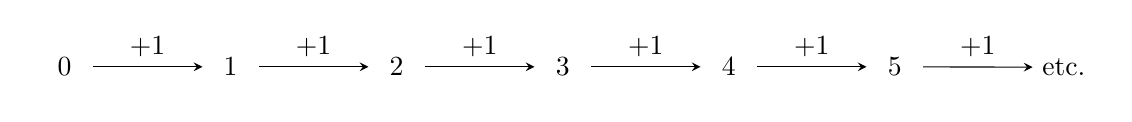
\begin{tikzpicture}
  \matrix (m) [matrix of math nodes,row sep=3em,column sep=4em,minimum width=2em]
  {
     0 & 1 & 2 & 3 & 4 & 5 & \text{etc.} \\};
  \path[-stealth]
    (m-1-1) edge node [above] {$+1$} (m-1-2)
    (m-1-2) edge node [above] {$+1$} (m-1-3)
    (m-1-3) edge node [above] {$+1$} (m-1-4)
    (m-1-4) edge node [above] {$+1$} (m-1-5)
    (m-1-5) edge node [above] {$+1$} (m-1-6)
    (m-1-6) edge node [above] {$+1$} (m-1-7);
\end{tikzpicture}
\end{center}
Similarly, one can get a list with elements in a set $C$ either by taking the empty list $[]$ or by taking the concatenation $c::l$ where $c \in C$ and $l$ is a list that has been previously built.\\
For example, the list $[a,b,a,a,a,b,a] = a::b::a::a::a::b::a::[]$ is obtained by $7$ concatenations done on the empty list.\\\\
Last example: one can get a binary tree by either taking only one leaf $\Leaf$ or by taking a node with a left tree and a right tree $\Node(L,R)$, both of the trees having been previously built.
For exemple, let us draw the tree $\Node(\Leaf,\Node(\Node(\Leaf,\Leaf),\Leaf))$: 
\begin{center}
\begin{tikzpicture}[scale=0.01]
  \matrix (m) [matrix of math nodes,row sep=3em,column sep=4em,minimum width=2em]
  { & \Node & & \\
    \Leaf & & \Node & \\
    & \Node & & \Leaf \\
    \Leaf & & \Leaf & \\};
  \path[-]
    (m-1-2) edge node {} (m-2-1)
    (m-1-2) edge node {} (m-2-3)
    (m-2-3) edge node {} (m-3-2)
    (m-2-3) edge node {} (m-3-4)
    (m-3-2) edge node {} (m-4-1)
    (m-3-2) edge node {} (m-4-3);
\end{tikzpicture}
\end{center}
These three data types are widely used in computer science, and it turns out that there is a good reason for this. Indeed, each of these data types can be seen as the initial algebra of some functor $F$. In addition to proving that these data types are mathematically canonical, this allows automatic factorization of other $F$-algebras.
\begin{center}
\begin{tabular}{|l|l|l|l|}
  \hline
  \gr{Data type} & Natural numbers & List of characters & Binary trees \\
  \hline
  \gr{Carrier} & $\N$ & $\List(C)$ & $\Tree$ \\
  & & & \\
  \gr{Elements} & $0$ & $[]$ & $\Leaf$ \\
  & $n+1$ & $c::l$ ($c \in C$) & $\Node(L,R)$ \\
  & & & \\
  \gr{Functor} & $F(A) = 1 + A$ & $F(A) = 1 + C \times A$ & $F(A) = 1 + A \times A$ \\
  & $F(f) = id_1 + f$ & $F(f) = id_1 + id_C \times f$ & $F(f) = id_1 + f \times f$ \\
  & & & \\
  \gr{Initial algebra} & $\iota : 1 + \N \to \N$ & $\iota : 1 + C \times \List(C)$ & $\iota : 1 + \Tree \times \Tree$ \\
  & $\iota(*) = 0$ & $\iota(*) = []$ & $\iota(*) = \Leaf$ \\
  & $\iota(n) = n+1$ & $\iota(c,l) = c::l$ & $\iota(L,R) = \Node(L,R)$ \\
  & & & \\
  \gr{Diagram} & $\lb \alpha \rb(0) = \alpha(*)$ & $\lb \alpha \rb([]) = \alpha(*)$ & $\lb \alpha \rb(\Leaf) = \alpha(*)$ \\
  & {\scriptsize $\lb \alpha \rb(n+1) = \alpha(\lb \alpha \rb(n))$} & {\scriptsize $\lb \alpha \rb (c::l)  = \alpha(c,\lb \alpha \rb(l))$} & {\scriptsize $\lb \alpha \rb (\Node(L,R)) = \alpha (\lb \alpha \rb (L) , \lb \alpha \rb (R))$} \\
  \hline
\end{tabular}
\end{center}
\end{document}

\newpage
\subsection*{Natural numbers}
According to the Peano axioms, there are two ways of obtaining a natural number. Either you take $0$, either you take the successor of some natural number $n$, written $n+1$. This is formalized by the following functor.
\begin{defi}
The functor $F : \gr{Set} \to \gr{Set}$ is defined by $F(A) = 1 + A$.
\end{defi}
In order to define a function on $1 + A$, we have to specify what is its value on $*$ and on every element of $A$. For example:
\begin{defi} $\iota : 1 + \N \to \N$ is defined by $\iota(*) = 0$ and $\iota(n) = n+1$. \end{defi}
\begin{theo} $\iota$ is the initial $F$-algebra. \end{theo} 
This means that for every morphism $\alpha : 1 + A \to A$, there is a unique morphism $\lb \alpha \rb : \N \to A$ such that the following diagram commutes.
\begin{center}
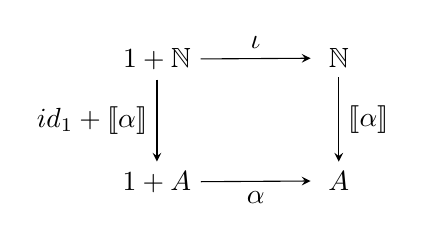
\begin{tikzpicture}
  \matrix (m) [matrix of math nodes,row sep=3em,column sep=4em,minimum width=2em]
  {
     1 + \N & \N \\
     1 + A & A \\};
  \path[-stealth]
    (m-1-1) edge node [left] {$id_1 + \lb \alpha \rb$} (m-2-1)
    (m-2-1) edge node [below] {$\alpha$}(m-2-2)
    (m-1-1) edge node [above] {$\iota$} (m-1-2)
    (m-1-2) edge node [right] {$\lb \alpha \rb$} (m-2-2);
\end{tikzpicture}
\end{center} 
Looking at the diagram, one sees that
\begin{itemize}
\setlength\itemsep{-0.3em}
\itemz $\lb \alpha \rb (0) = \alpha(*)$
\itemz $\lb \alpha \rb (n+1) = \alpha(\lb \alpha \rb (n))$
\end{itemize}
Hence $\lb \alpha \rb(n) = \alpha^n(*)$. The morphism $\lb \alpha \rb$ is formalizing the type of induction that natural numbers stand for, i.e., one-directional, repeated application of the same function.
\begin{center}
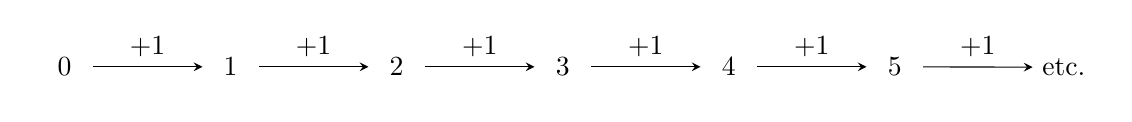
\begin{tikzpicture}
  \matrix (m) [matrix of math nodes,row sep=3em,column sep=4em,minimum width=2em]
  {
     0 & 1 & 2 & 3 & 4 & 5 & \text{etc.} \\};
  \path[-stealth]
    (m-1-1) edge node [above] {$+1$} (m-1-2)
    (m-1-2) edge node [above] {$+1$} (m-1-3)
    (m-1-3) edge node [above] {$+1$} (m-1-4)
    (m-1-4) edge node [above] {$+1$} (m-1-5)
    (m-1-5) edge node [above] {$+1$} (m-1-6)
    (m-1-6) edge node [above] {$+1$} (m-1-7);
\end{tikzpicture}
\end{center} 
\newpage
\subsection*{Lists}
Remember what a list is in computer science. First, it is a list \il{of something}. We choose to look at lists of \il{characters}, i.e., each element of a list is a character living in a set of characters $C$. How do we define a list of characters in computer science ? Either it is the empty list, denoted by $[]$, or it is the concatenation of one character $c$ and a list $l$, denoted by $c::l$. In your opinion, what will be the functor that will be useful to model this situation?
\begin{defi}
The functor $F : \gr{Set} \to \gr{Set}$ is defined by $F(A) = 1 + C \times A$. If $f : A \to B$ is a function then $F(f) = id_1 + id_C \times f$ is the function defined by $F(f)(*) = *$ and $F(f)(c,a) = (c,f(a))$ for any $(c,a) \in C \times A$.
\end{defi}
In order to define a function on $1 + C \times A$, we have to specify what is its value on $*$ and on every element of $C \times A$. Let us take $A = \List(C)$ the set of lists of characters in $C$ (for example, if $C = \{a,b\}$, $\List(C) = \{[], [a], [b], [a,b], [a,a], [b,b], [b,a], [a,a,b], [a,b,a], [a,a,b,a,b,b,b]...\}$). Then we define the following $F$-algebra.
\begin{defi} $\iota : 1 + C \times \List(C) \to \List(C)$ is defined by $\iota(*) = []$ (the empty list) and $\iota(c,l) = c::l$.\end{defi}
\begin{theo} $\iota$ is the initial $F$-algebra. \end{theo} 
This means that for every morphism $\alpha : 1 + C \times A \to A$, there is a unique morphism $\lb \alpha \rb : \List(C) \to A$ such that the following diagram commutes.
\begin{center}
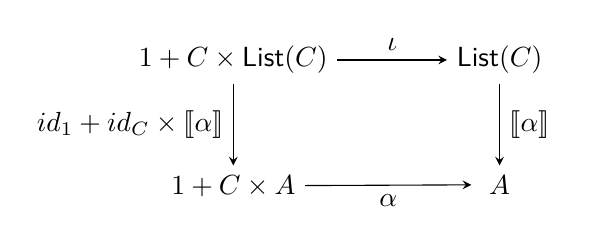
\begin{tikzpicture}
  \matrix (m) [matrix of math nodes,row sep=3em,column sep=4em,minimum width=2em]
  {
     1 + C \times \List(C) & \List(C) \\
     1 + C \times A & A \\};
  \path[-stealth]
    (m-1-1) edge node [left] {$id_1 + id_C \times \lb \alpha \rb$} (m-2-1)
    (m-2-1) edge node [below] {$\alpha$}(m-2-2)
    (m-1-1) edge node [above] {$\iota$} (m-1-2)
    (m-1-2) edge node [right] {$\lb \alpha \rb$} (m-2-2);
\end{tikzpicture}
\end{center} 
Looking at the diagram, one sees that
\begin{itemize}
\setlength\itemsep{-0.3em}
\itemz $\lb \alpha \rb ([]) = \alpha(*)$
\itemz $\lb \alpha \rb (c::l) = \alpha(c,\lb \alpha \rb(l))$
\end{itemize}
There is no simple expression for $\lb \alpha \rb$. The morphism $\lb \alpha \rb$ is formalizing the type of induction that lists stand for. The fact that the initial $F$-algebra is precisely the algebra of lists means that lists are a very canonical structure. 
\newpage
\subsection*{Binary trees}
A binary tree $T$ is either a leaf $\Leaf$ or composed of a node and two  binary trees $L,R$ ($L$ is the left sub-tree and $R$ is the right sub-tree). It is denoted by $\Node(L,R)$ and represented by
\begin{center}
\begin{tikzpicture}
  \matrix (m) [matrix of math nodes,row sep=3em,column sep=4em,minimum width=2em]
  {
     & \Node & \\
     L & & R \\};
  \path[-]
    (m-1-2) edge node [above left] {} (m-2-1)
    (m-1-2) edge node [above right] {} (m-2-3);
\end{tikzpicture}
\end{center}
For exemple, let us draw the tree $\Node(\Leaf,\Node(\Node(\Leaf,\Leaf),\Leaf))$: 
\begin{center}
\begin{tikzpicture}
  \matrix (m) [matrix of math nodes,row sep=3em,column sep=4em,minimum width=2em]
  { & \Node & & \\
    \Leaf & & \Node & \\
    & \Node & & \Leaf \\
    \Leaf & & \Leaf & \\};
  \path[-]
    (m-1-2) edge node {} (m-2-1)
    (m-1-2) edge node {} (m-2-3)
    (m-2-3) edge node {} (m-3-2)
    (m-2-3) edge node {} (m-3-4)
    (m-3-2) edge node {} (m-4-1)
    (m-3-2) edge node {} (m-4-3);
\end{tikzpicture}
\end{center}
\begin{defi}
The functor $F : \gr{Set} \to \gr{Set}$ is defined by $F(A) = 1 + A \times A$. If $f : A \to B$ is a function then $F(f) = id_1 + f \times f$ is the function defined by $F(f)(*) = *$ and $F(f)(a,a') = (f(a),f(a'))$ for any $(a,a') \in A \times A$.
\end{defi}
Let $\Tree$ be the set of all binary trees.
\begin{defi} $\iota : 1 + \Tree \times \Tree \to \Tree$ is defined by $\iota(*) = \Leaf$ and $\iota(L,R) = \Node(L,R)$.
\end{defi}
\begin{theo}
$\iota$ is the initial $F$-algebra.
\end{theo}

This means that for every morphism $\alpha : 1 + A \times A \to A$, there is a unique morphism $\lb \alpha \rb : \Tree \to A$ such that the following diagram commutes.
\begin{center}
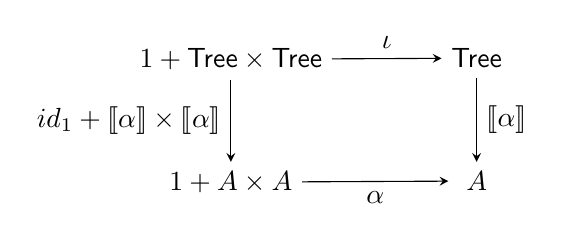
\begin{tikzpicture}
  \matrix (m) [matrix of math nodes,row sep=3em,column sep=4em,minimum width=2em]
  {
     1 + \Tree \times \Tree & \Tree \\
     1 + A \times A & A \\};
  \path[-stealth]
    (m-1-1) edge node [left] {$id_1 + \lb \alpha \rb \times \lb \alpha \rb$} (m-2-1)
    (m-2-1) edge node [below] {$\alpha$}(m-2-2)
    (m-1-1) edge node [above] {$\iota$} (m-1-2)
    (m-1-2) edge node [right] {$\lb \alpha \rb$} (m-2-2);
\end{tikzpicture}
\end{center} 
Looking at the diagram, one sees that
\begin{itemize}
\itemz $\lb \alpha \rb (\Leaf) = \alpha(*)$
\itemz $\lb \alpha \rb (\Node(L,R)) = \alpha(\lb \alpha \rb(L) , \lb \alpha \rb(R))$
\end{itemize}
\end{document}